\documentclass[11pt]{article}

\def\articlename{资产定价}
\def\authorname{杨弘毅}
\def\startdate{2021年6月10日}

\ifx \authorname\undefined
  \def\authorname{杨弘毅}
\else
\fi

\author{\authorname}
\date{创建:\startdate \\修改:\today}

\usepackage[a4paper,left=6em,right=6em]{geometry}
\usepackage{amsmath,amsfonts,amsthm,bbold}
\usepackage{booktabs,float,multirow}
\usepackage{cancel}
\usepackage{enumitem}
\usepackage{multicol}
\usepackage{graphicx}
\usepackage[toc,title]{appendix}
\usepackage{tikz}
\usetikzlibrary{arrows.meta}
\usetikzlibrary{patterns}
\usetikzlibrary{decorations.pathreplacing}
\usetikzlibrary{decorations.pathmorphing}
\usepackage{subcaption}
\usepackage{fancyhdr}
\pagestyle{fancy}
\setlength{\headheight}{15pt}
\usepackage{footmisc}
\usepackage{hyperref}
\usepackage{tocloft}
\hypersetup{
    colorlinks=true, %set true if you want colored links
    linkcolor=blue,
    linktoc=all, %set to all if you want both sections and subsections linked
    citecolor=black,
    filecolor=black,
    urlcolor=blue
}
\usepackage[UTF8]{ctex}

\title{\articlename}

% Format
\setlength{\cftbeforesecskip}{6pt}
\setlength{\parskip}{0.6em}
\renewcommand{\baselinestretch}{1.4}
\setlist{noitemsep,itemindent=1em,topsep=0em,leftmargin=4em,rightmargin=4em}
\setlist[2]{leftmargin=2em}

% Shortcut
\newcommand{\divider}{\vspace{-\parskip}\noindent\rule{\linewidth}{0.4pt}}
\newcommand{\tops}[1]{\texorpdfstring{#1}{TEXT}}

% Theorem
\newtheorem{thm}{定理}[section] 
\newtheorem{proposition}[thm]{命题}
\newtheorem{lemma}[thm]{引理}
\newtheorem{corollary}[thm]{推论}
\newtheorem{property}[thm]{性质}
\newtheorem{example}[thm]{例子}
\newtheorem{remark}[thm]{备注}
\newtheorem{note}[thm]{注释}

% Symbol
\newcommand{\E}{\mathbb{E}}
\newcommand{\mcl}{\mathcal{L}}
\newcommand{\rnE}{\widetilde{\mathbb{E}}}
\newcommand{\wt}[1]{\widetilde{#1}}
\DeclareMathOperator{\Var}{Var}
\DeclareMathOperator{\Cov}{Cov}
\newcommand{\abs}[1]{\left\lvert #1\right\rvert}
\newcommand{\norm}[1]{\left\lVert #1\right\rVert}
\newcommand{\given}{\:\vert\:}

\begin{document}
\maketitle
\tableofcontents

\section{TODO}
\begin{itemize}
    \item campbell-shiller分解
\end{itemize}

\section{基础}

\subsection{CAPM与APT}

资本资产定价模型(Capital Asset Pricing Model,CAPM)的诞生,才首次清晰的描绘出风险与收益率之间的关系。根据CAPM模型,资产的预期超额收益率由如下一元线性方程决定:
\begin{equation*}
    \E[R_i] - R_f = \beta_i \left( \E[R_M]-R_f \right)
\end{equation*}

其中$R_i$为某资产$i$的收益率,$R_f$为无风险收益率,$\E[R_M]$为市场组合的预期收益率,$\E[R_m]- R_f$为市场风险溢价(Market risk premium),也称为市场因子。其中有$\beta_i = \frac{\Cov(R_i,R_M)}{\Var(R_M)}$,$\beta$刻画了该资产$i$收益对于市场收益的敏感程度,也被称为资产$i$对市场风险的暴露程度。

随后Ross(1976)提出了著名的套利定价理论(Arbitrage Pricing Theory,APT),为多元线性模型:
\begin{equation*}
    \E[R_i^e] = \bm{\beta_{i}^{'} \lambda}
\end{equation*}

同CAPM模型相同,$\bm{\beta}$为因子暴露(Factor exposure)或称为因子载荷(Factor loading),$\bm{\lambda}$是因子预期收益率(Factor expected return),或称为因子溢价(Factor risk premium)或因子风险溢酬。由此可见,资产$i$的预期超额收益率$\E[R_i^e]$,为等式右侧一系列因子的预期收益率,以及该资产在这些因子上的暴露决定。

此时研究的是不同资产之间的预期超额收益率的差别,称为(横)截面(Cross-sectional)差异,而非时间序列(Time-series)或时序上的差异。因子代表了收益率的一种结构,给定了结构与因子预期收益率,不同资产预期超额收益率的差别,由其在这些因子上的暴露决定。\uline{那么多因子模型研究的核心问题,是找到一组能够解释股票预期收益率界面差异的因子}。

\begin{figure}[H]
    \centering
    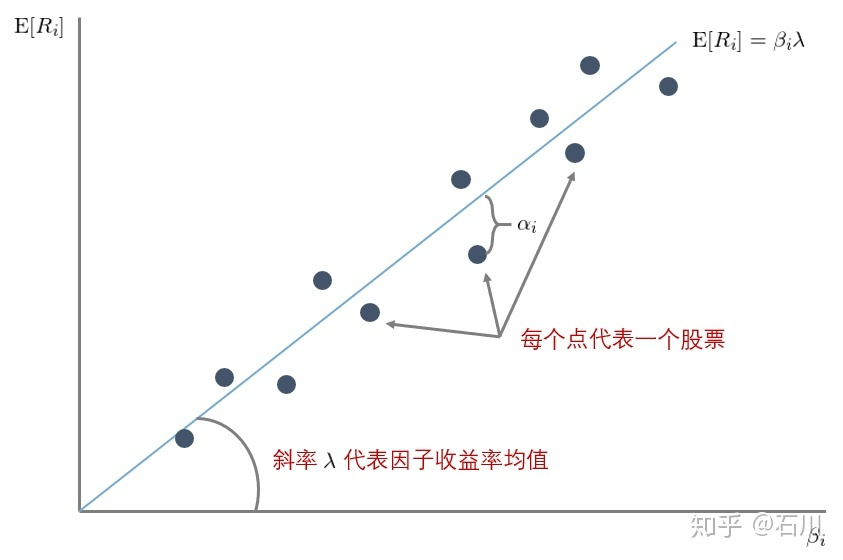
\includegraphics[width=0.6\textwidth]{fig/capm_sml.jpg}
    \caption{CAPM:Security Market Line}
    \label{fig:sml}
\end{figure}

有几点需要注意,在这里使用$\E[\bm{R_i^e}]$为代表资产的预期超额收益率,而非如CAPM中表示的$\E[R_i] - R_f$,是因为在实证中,经常采用多空对冲建立投资组合,此时便无需再减去无风险收益率。另外,学界研究的对象始终为资产的预期草娥收益,因此有时将“超额”二字省略。

\subsection{异象}

而在实际过程中,等式两侧并不相等,而存在着定价误差$\alpha_i$(Pricing error):
\begin{equation*}
    \E[R_i^e] = \alpha_i + \bm{\beta_{i}^{'} \lambda}
\end{equation*}

定价误差有可能由两方面产生:
\begin{itemize}
    \item 模型设定偏误,即等式右侧遗漏了重要的因子,当被遗漏因子加入后,可消除定价误差
    \item 模型设定没有问题,但由于资产收益的实际数据只是总体的一个样本,那么误差总是存在的,此时需要通过统计的方法检验误差$\alpha_i$是否显著不为零:
    \begin{itemize}
        \item 若$\alpha_i$并非显著偏离于零,则出现只是样本问题
        \item 若$\alpha_i$\textbf{显著偏离零},则说明了可以通过套利而获得超额收益的机会,市场对该资产出现错误定价(Mispricing),从而导致了实际预期收益率与多因子模型下的预期收益率出现偏离
    \end{itemize}
\end{itemize}

假使我们根据基本面特征或量价指标等特征,挑选出一揽子股票并构建\uline{多空投资组合}。若该组合的收益率无法被多因子模型(如3因子、4因子、5因子模型)解释,则称该特征为一个\textbf{异象}(Anomaly)。即该特征获得了多因子模型无法解释$alpha$收益率,但从有效市场假说出发,市场中不应该存在很多异象。同时在学界不断的挖掘中,获得了400+个异象,且在样本内都获得了很高的t-statistics,这里可能存在两个原因:
\begin{itemize}
    \item 数据挖掘,大量的异象在样本内被挖掘出,因此Harvey,Liu和Zhu(2016)提出异象收益率的t-statistic至少要超过3.0,而非传统的5\%显著性对应的2.0,才可能真正有效,而非来源于运气
    \item 模型相关,若以$CAPM$为定价模型,那么许多异象都能获得CAPM无法解释的$\alpha$收益率,同时随着定价模型中因子个数的增加,更多的异象变得不再显著,而真正的定价模型是未知的
\end{itemize}

Hou,Xue和Zhang(2017)长达146页对异象的研究中,复现了学术界提出的 447 个异象,涵盖动量(57个)、价值/成长(68个)、投资(38个)、盈利(79个)、无形资产(103个)、以及交易摩擦(102个)六大类。对于这447个异象,在排除了微小市值股票的影响后,其中286个(64\%),在5\%的显著性水平下不再显著(下同)。若按照Harvey,Liu和Zhu(2016)的建议把t-statistic的阈值提升到3.0,其中380个(85\%)异象不再显著。最后,如果使用Hou,Xue和Zhang(2015)提出的4因子模型作为定价模型,那么其中436个(98\%)异象不再显著,仅有 11个异象显著。

对于超额收益,学术界和业界主流的两种解释是错误定价和风险补偿,错误定价意味着投资者可以通过合理的策略获得潜在的超额收益;而风险补偿则意味着投资者获得的收益是以承担额外风险为代价的。

\subsection{因子}

异象有可能能成为优秀的因子,但不是所有异象都是因子。因为作为一个因子(Factor),需要能够解释资产(个股或投资组合)预期收益率截面上的差异,并有增量贡献。具体而言:
\begin{itemize}
    \item 异象从方程的左侧,移动到右侧称为一个因子,称为解释变量,需要考察期是否能解释预期收益率截面上的差异
    \item 由于多个异象之间并不完全独立,需要排除相关性的影响,考察是否有增量贡献
\end{itemize}

如价值因子,也可以采用$E/P$或$B/P$构建High-Minus-Low组合,若同时使用,两者相关性必然很高,因此若使用其一作为价值因子,另一因子对资产预期收益率截面差异的解释能力的增量贡献将变得很低,无法称为因子。

对于因子模型接下去的问题就是,在构建多因子模型时:选取因子因子的数目;以及选取哪些因子。第一个问题,因遵循简约法则(The Law of Parsimony),或奥卡姆剃刀(Occam's razor)。若从ICAPM(Intertemporal CAPM)的角度理解多因子模型,每个因子应代表某种状态变量(State variable),即为投资者想要对冲的某种风险。因此,因子的个数应该是有限的。目前主流的多因子模型如下:
\begin{itemize}
    \item Fama-French 三因子模型(Fama and French 1993):多因子模型的开山鼻祖,包括MKT、HML以及SMB三因子。其中包含了MKT市场因子,HML价值因子,与SMB规模因子
    \item Carhart 四因子模型(Carhart 1997):在 Fama-French三因子模型上加上了动量MOM因子。
    \item Novy-Marx四因子模型(Novy-Marx 2013):包含MKT,HML,MOM以及PMU四个因子,其中 PMU 所用的财务指标是Gross Profit-to-Asset,代表Profitability维度
    \item Fama-French 五因子模型(Fama and French 2015):Fama和French在其三因子模型的基础上加入了CMA和RMW两个因子,分别代表Investment和Profitability 两个维度。
    \item Hou-Xue-Zhang 四因子模型(Hou, Xue and Zhang 2015):包含MKT,SMB,IVA以及ROE。其中IVA是Total assets的年增长率,代表Investment 维度
    \item Stambaugh-Yuan四因子模型(Stambaugh and Yuan 2016):包含MKT,SMB,MGMT和PERF四个因子。MGMT和PERF分别使用了6个和5个指标,代表Management以及 Performance相关的两个Mispricing因子。虽然该模型只有四个因子,但它用到的基本面和量价指标多达 12 个。
    \item Daniel-Hirshleifer-Sun三因子模型(Daniel, Hirshleifer and Sun 2018):在MKT的基础上,使用PEAD和FIN两个指标作为短期和长期行为因子(Behavioral factors)的代理指标,构建了三因子模型。该模型由于包括了传统的MKT市场因子,又包括行为因子,故称为复合模型。
\end{itemize}

对于第二个问题,则涉及了不同多因子模型之间的比较。目前学界主要有三种方法:
\begin{itemize}
    \item GRS tests
    \item Mean-Variance Spanning tests
    \item Bayesian approach
\end{itemize}

【待整理】

GRS tests(Gibbons,Ross和Shanken 1989)检验n个资产在给定因子模型下的定价错误$\alpha$,是否在统计上联合为零(jointly equal to zero)。在比较两个多因子模型时,使用两个模型的因子互为资产和定价模型进行检验。

Mean-Variance Spanning tests考察n个已知资产构建的mean-variance有效前沿能否包含某个新资产(Huberman和Kandel 1987)。在比较两个多因子模型时,使用每个模型的因子构建有效前沿,并逐一检验其能否包含另一个模型中的因子。

在Bayesian approach中,假设比较两个多因子模型$M_1$和$M_2$,数据集使用$D$表示。令 $P(M_1)$和$P(M_2)$为这两个模型的先验概率,且有$P(M_1) + prob(M_2) = 1$(这里假设把多个模型两两比较)。根据贝叶斯定理有:
\begin{equation*}
    P(M_i \given D) = \frac{P(M_i)P(D \given M_i)}{P(M_1)P(D\given M_1) + P(M_2)P(D\given M_2)}
\end{equation*}

其中:
\begin{equation*}
    P(D \given M_i) = \int_{\theta_i} P(\theta_i) P(D \given \theta_i) d\theta_i
\end{equation*}

上式中,$P(\theta_i)$是模型$i$参数的先验分布,$P(D \given \theta_i)$是模型$i$的似然函数。上述贝叶斯方法的核心在于确定$P(\theta_i)$。根据Pastor和Stambaugh(2000) 以及Barillas和Shanken(2018)的理论,它和以两个模型中的全部因子作为资产所构成的投资组合的预期最大夏普率的平方与市场夏普率的比值有关。

\subsection{系统性风险}

【待整理】

除了市场因子以外的风险都是可以被分散的,所以只要是超过市场组合收益的部分都叫做超额收益。

多因子模型的表达式同样强调,只有那些影响众多资产收益率共同运动的风险,而非资产的特质性风险(即可以通过分散化规避掉的风险),才是预期收益率的来源。

系统风险(Systematic risk)的暴露程度,即对于市场风险暴露的大小。即资产的预期超额收益率,由市场组合(市场因子)的预期超额收益率与该资产对市场风险的暴露大小决定。或可以理解为,单项资产的$\beta$系数是指资产预期超额收益率与市场组合预期超额收益率之间变动关系的敏感程度。

系统性风险(Systematic risk),又称市场风险或不可分散风险,是影响所有资产的、不能通过资产组合而消除的风险。这部分风险是由那些影响整个市场的风险所引起的,无论怎样分散投资,也不可能消除系统性风险。避免集中投资于单一市场可减少系统性风险。单项资产、证券资产组合或不同公司受系统性风险影响不一样,系统性风险的大小通常用beta系数($\beta$系数)来衡量。

\section{多因子模型回归检验}

对于多因子截面关系式:
\begin{equation*}
    \E[R_i] = \alpha_i + \bm{\beta_{i}^{'} \lambda}
\end{equation*}

在上述截面关系式中,$\alpha_i$代表股票i的定价错误。如果我们能够在统计上证明所有股票的$\alpha_i$都很接近零,那么这个多因子模型就是很好的模型。因为这些因子能够较好的解释个股截面预期收益率的差别。因此,多因子模型的回归检验中的重中之重,就是所有这些$\alpha_i$联合起来是否在统计上足够接近零。

因此,多因子模型的回归检验可以总结为:
\begin{itemize}
    \item 挑选因子,计算个股在这些因子上的暴露$\beta_i$
    \item 找到个股超额收益率均值$\E[R_i]$和因子暴露$\beta_i$在截面上的关系
    \item 计算个股的定价误差$\alpha_i$,联合检验这些$\alpha_i$是否在统计上为零
\end{itemize}

https://zhuanlan.zhihu.com/p/40984029

注意:超额收益率为t+1期,而因子为t期,由于对于所有股票,无风险利率相同,不会影响beta。

\subsection{时序回归}

此时的因子为投资组合收益率,如经典的HML,SMB等,那么此时可以通过时序回归,来分析个股超额收益率$\E[R_i]$与因子暴露$\beta_i$之间在截面上的关系。

对于个股i,直接进行时间序列回归,即
\begin{equation*}
    R_{i,t} = \alpha_i + \bm{\beta_{i}^{'} f_t} + \varepsilon_{i,t} \inlinesep t=1,2,\dots,T
\end{equation*}

对$R_{i,t}$与$f_t$在时序上取均值$\E_T(\cdot)$,就得到了个股超额收益率与因子暴露在截面上的关系:
\begin{equation*}
    \E_T[R_i] = \alpha_i + \bm{\beta_{i}^{'}} \E_T[\bm{f_t}] \inlinesep t=1,2,\dots,T
\end{equation*}

此时时序回归得到的截距$\alpha_i$即为个股i的定价误差。Black,Jensen和Scholes(1972) 基于如上的论述给出了时序回归法中求解因子预期收益率的简单方法,因子收益率$f_t$,在时序上的均值就是因子的预期收益率:
\begin{equation*}
    \bm{\lambda} = \E_T[\bm{f}]
\end{equation*}

对于N支个股,每支个股i都有一组$(\beta_i,\E[R_i])$,以$\E[R_i] = \bm{\beta'} \E[\bm{f}]$作图,此时斜率为因子收益率$\lambda=\E_T[\bm{f}]$。将当$\bm{\beta_i}=0$时与$\bm{\beta_i}=1$代入,可知该直线过$(0,0)$与$(1,\E[\bm{f}])$两点。即对于因子投资组合,其对自身的因子暴露为1。

\begin{figure}[H]
    \centering
    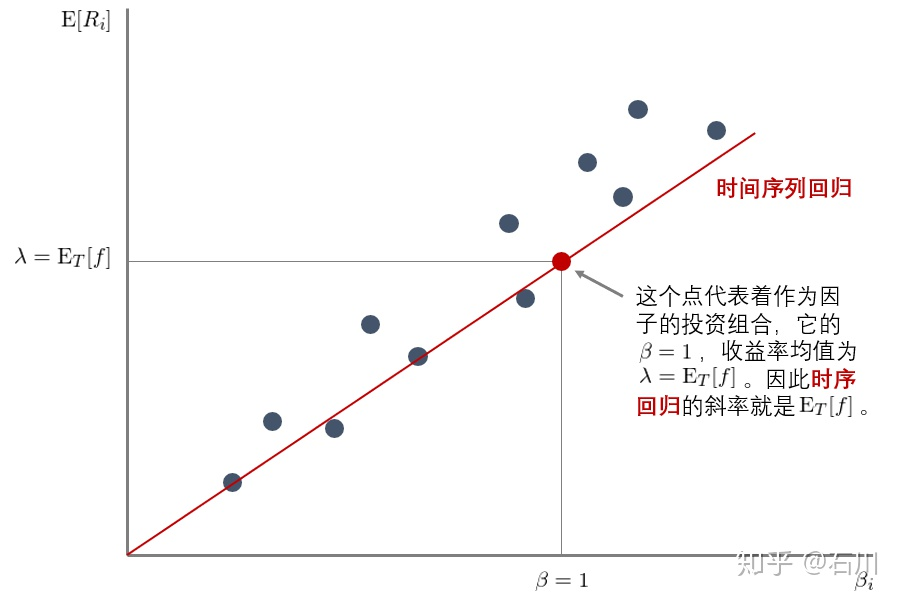
\includegraphics[width=0.8\textwidth]{fig/ts_reg.jpg}
    \caption{时序回归}
    \label{fig:ts_reg}
\end{figure}

对于检验$\alpha_i$联合起来是否统计上为零,若残差不相关和同方差,标准误可以由OLS标准公式计算。若残差满足独立同分布且为正态分布,可以使用GRS检验。而当残差之间存在相关性或者异方差,则需要使用GMM。

\subsection{截面回归}

相比于时序回归,使用截面回归的优势是,因子的选择范围更广。可以为GDP、CPI、利率等宏观经济指标,而不仅投资组合收益率。进行截面回归,首先需先进行时序回归,用于确定因子暴露$\bm{\beta}$,即个股收益率对这些因子在时序上的敏感程度。对于个股i,应有:
\begin{equation*}
    R_{i,t} = a_i + \bm{\beta_{i}^{'} f_t + \varepsilon_{i,t}} \inlinesep t=1,2,\dots,T
\end{equation*}

由于此时的$\bm{f_t}$并非个股收益率,阶矩$a_i$并非个股定价误差。得到了个股因子暴露$\beta$之后,再进行截面回归。此时等式左边为$\E_T[R_i]$为整个T其的收益率均值,或上述$\E_T[R_i]$,而右侧为时序回归得到的$\bm{\beta_i}$。对于n支个股,每支个股都有一组$(\E[R_i],\bm{\beta_i})$,则截面回归的表达式为:
\begin{equation*}
    \E[R_i] = \alpha_i + \bm{\beta_{i}^{'} \lambda}
\end{equation*}

此时的截距即为定价误差,但由于只进行了一次回归,因此只能得到\uline{单个}定价误差$\alpha_i$与\uline{单个}因子预期收益率$\bm{\lambda}$。

\begin{figure}[H]
    \centering
    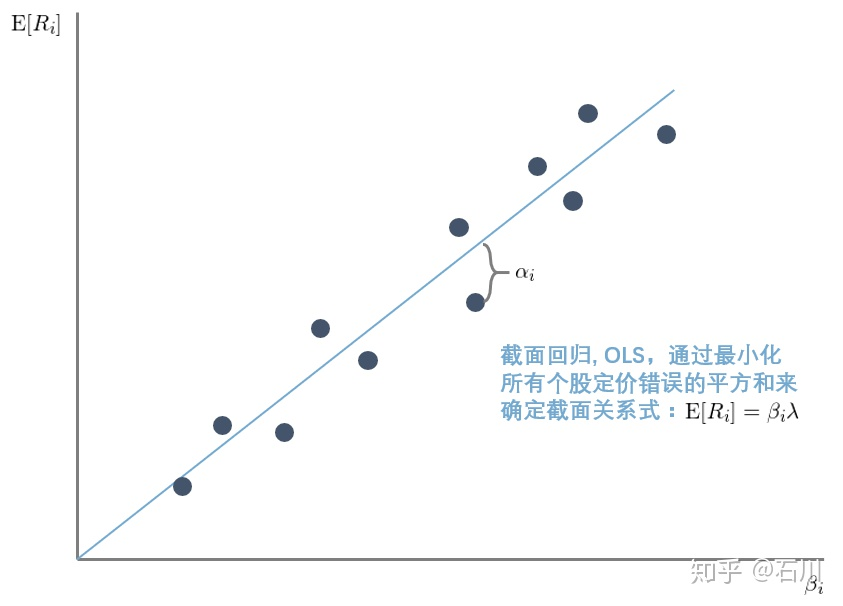
\includegraphics[width=0.8\textwidth]{fig/cs_reg.jpg}
    \caption{截面回归}
    \label{fig:cs_reg}
\end{figure}

因此截面回归,也称为Two-pass regression estimate。即通过时序回归首先得到个股对因子的暴露,以及收益率均值。即将个股转换为一个点$(\beta_i,\E[R_i])$,再对n支个股进行截面回归,最终的到定价误差与因子收益率。

由于截面个股残差的相关性,虽然不会影响OLS估计,但会导致OLS给出的标准误存在较大误差,因此可以使用GLS取代OLS,由于GLS考虑了残差的协方差因此可以得到准确的标准误。但估计残差的协方差矩阵在现实中有较大的障碍。此时则可使用GMM,由于截面回归的$\bm{beta_i}$并不是使用真实的因子收益率回归得到,而是从时间序列上回归出的估计值,称为generated regressors,存在误差。Shanken(1992)给出了修正方法称为Shanken correction。同时利用Shanken correction与GMM,即可检验$\alpha_i$是否联合为0。

\subsection{时序回归 vs 截面回归}

对于时序回归而言,因子收益率为在时序上的均值,即$\bm{\lambda} = \E_T[\bm{f}]$,来得到隐含的截面关系。因此$\E[R_i] = \bm{\beta_i \lambda}$必然过原点,以及因子收益率的投资组合$(1,\E_T[\bm{f}])$($\bm{\beta_i}=2$)。而在截面回归中,因子暴露已经通过时序回归确定,而在第二次进行截面回归时,充分使用了个股数据,若使用OLS,以最小化个股定价误差$\alpha_i$的平方和为目标。因子收益率与时序中直接通过计算均值的方式不同,更加合理。

\begin{figure}[H]
    \centering
    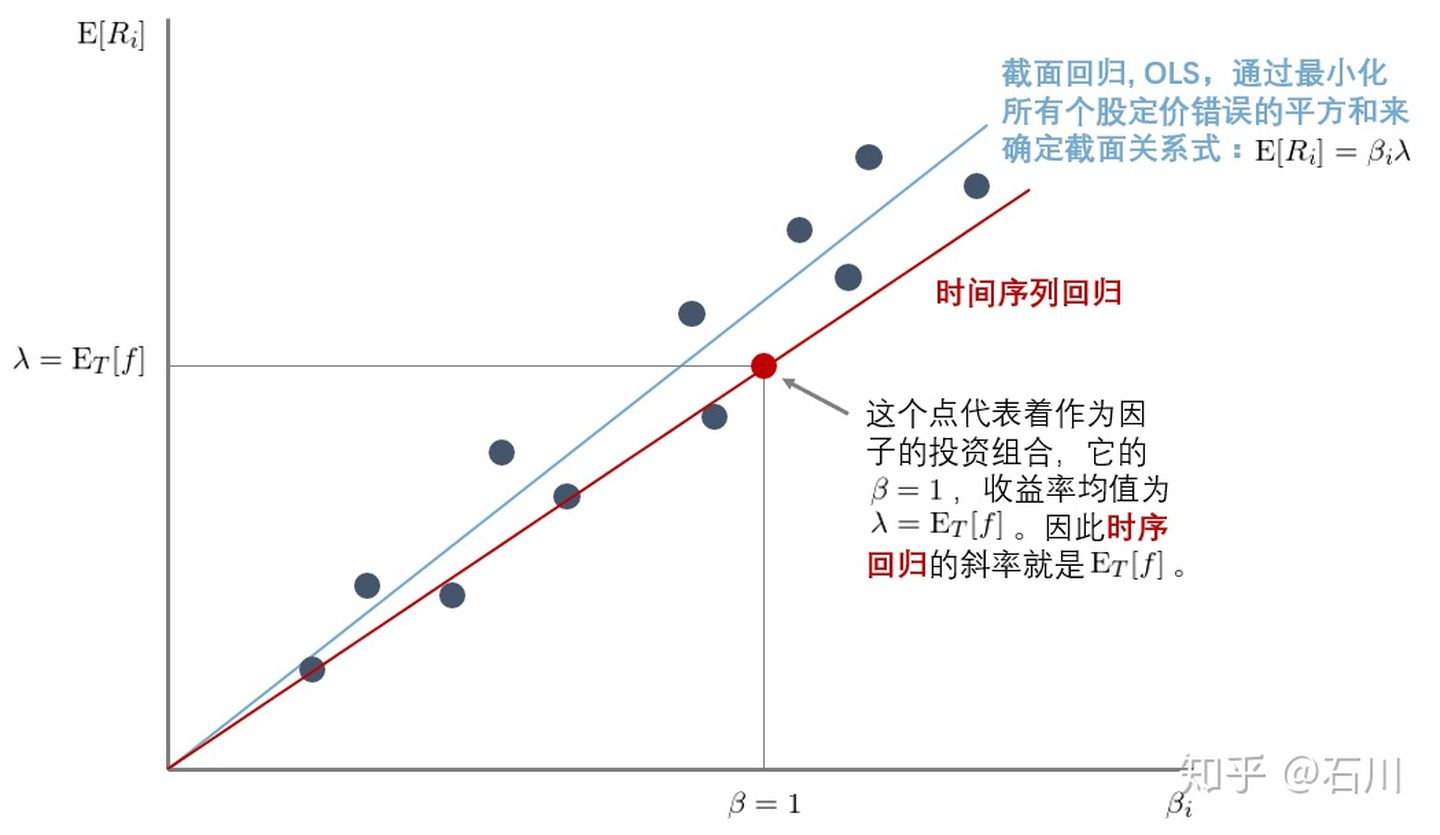
\includegraphics[width=0.8\textwidth]{fig/ts_vs_cs.jpg}
    \caption{时序回归与截面回归}
    \label{fig:ts_vs_cs}
\end{figure}

\subsection{Fama-MacBeth回归}

在Fama和MacBeth(1973)中,提出了Fama-MacBeth Regression(Fama and MacBeth 1973),目的是为了检验 CAPM。首先,与截面回归相同,也需要先进行时序回归,得到个股收益率在因子收益率上的暴露$\beta_i$。其次,与截面回归不同的是,Fama-MacBeth在每个t时间上进行一次截面回归。在截面回归中,对资产i,在时序$t=1,2,\dots,T$上对$\R_{i,t}$取均值,得到$\E[R_i]$。与该资产i的因子暴露$\bm{beta}_i$进行回归,注意这里只进行了\uline{1次回归}:
\begin{equation*}
    \E[R_i] = \alpha_i + \bm{\beta_{i}^{'} \lambda_i}
\end{equation*}

对于Fama-MacBeth回归,具体而言,并不对$R_{i,t}$取均值,而对每个t时刻都进行一次独立的截面回归,一共进行\uline{T次回归}:
\begin{equation*}
    R_{i,t} = \alpha_{i,t} + \bm{\beta_{i}^{'} \lambda_t}
\end{equation*}

那么此时对于$\alpha_{i,t}$与$\lambda_t$都有T次回归结果。对于单个资产i,从$t=1$时刻到$t=T$时刻,有$\left(\bm{\beta_{i,1}},\E[R_{i,1}]\right),\left(\bm{\beta_{i,2}},\E[R_{i,2}]\right),\dots,\left(\bm{\beta_{i,T}},\E[R_{i,T}]\right)$。即可以以此估计定价误差以及因子收益率:
\begin{align*}
    \hat{\lambda} &= \frac{1}{T} \sum_{t=1}^{T} \lambda_t \\
    \hat{\alpha}_i &= \frac{1}{T} \sum_{t=1}^{T} \alpha_{i,t}
\end{align*}

不同于传统截面回归,只得到$\lambda$和$\alpha$的一个样本估计,在FM截面回归中得到T个$\lambda$和$\alpha$的样本估计,这样就可以求出两者标准误为:
\begin{align*}
    \sigma^2(\hat{\lambda}) &= \frac{1}{T^2} \sum_{t=1}^{T} \left( \hat{\lambda}_t - \hat{\lambda} \right)^2 \\
    \sigma^2(\hat{\alpha}_i) &= \frac{1}{T^2} \sum_{t=1}^{T} \left( \hat{\alpha}_{i,t} - \hat{\alpha}_i \right)^2
\end{align*}

Fama-MacBeth截面回归和传统截面回归的相同点和区别是:
\begin{itemize}
    \item FM回归与截面回归,都需先进行时序回归,以确定个股的因子暴露$\bm{\beta_i}$
    \item 传统截面回归将$R_{i,t}$在时序上取均值得到$\E[R_i]$,再进行1次截面回归,得到$\alpha_i$和$\lambda$
    \item 对于FM回归,在各个不同的t时刻使用$R_{i,t}$与$\bm{\beta_{i}}$进行回归,再将回归结果在时序上取均值得到$\alpha_i = \E[\alpha_{i,t}]$与$\lambda=\E[\lambda_t]$
\end{itemize}

在Fama和MacBeth(1973)中,在时序上采用了滚动窗口的方法估计$\bm{\beta_i}$,因此对于不同的t,$\bm{\beta_i}$发生改变。若使用所有样本一次性估计$\bm{\beta_i}$,那么取值相同。此时由于$\bm{\beta_i}$不变,那么对于传统截面回归的先均值再回归,与FM截面回归的先回归再均值,两种方式在所有T期上得到的估计是相同的,但FM截面回归仍然有一定的优势。

【待整理】
由上面的介绍可知,Fama-MacBeth 回归的最大优点是它排除了残差截面相关性对标准误的影响。股票的残差收益率在截面上具有很高的相关性,因此该修正对于准确计算标准误至关重要。下面来说说它的不足。首先,Fama-MacBeth 回归对于残差在时序上的相关性无能为力。如果残差在时序上存在相关性,则需要对 Fama-MacBeth 回归得到的标准误进一步修正。Petersen (2009) 分析了不同的回归技术在分析面板数据(panel data)时由于忽略残差的时序或截面相关性而导致不准确的标准误(低估了其真实值)。这篇文章非常值得一读。其次,上文提到,在截面回归中用到的$\bm{\beta_i}$并不是已知的,而是通过时间序列得到的估计值(generated regressors),因此存在误差。Fama-MacBeth 回归对此也无能为力,需要 Shanken correction。

\subsection{Barra多因子模型}

Barra多因子模型也是截面回归模型,其考虑了行业因子和来自基本面和技术面的风格因子。但与传统的截面回归模型不同的是在Barra模型中,因子暴露并非来自时间序列回归,而是直接来自基本面或者技术面数据本身。

例如Book-to-Market ratio,在Fama-French三因子模型中,其被用来构建HML(High-Minus-Low)投资组合,投资组合的收益率作为因子。由时序回归决定个股在这个因子上的暴露,与个股实际的BM无关。但在Barra模型中,BM直接用于确定因子暴露,但需要进行标准化。有了因子暴露,Barra截面模型与传统截面模型相同,都是通过截面回归确定因子收益率。因此,Barra 模型(业界代表)和学术界流行的因子模型最大的不同就是因子暴露$\bm{\beta_i}$的确定。

对于两种确定因子暴露的方法,通过时间序列得到的$\bm{\beta}$,经过平滑,变化更加缓慢。而直接使用基本面数据获得$\bm{\beta}$,可以更快的捕捉公司的变化。需要注意的是,这些因子都需要进行标准化,不能直接使用原始数据。例如,公司市值不经过标准化而作为因子暴露,公司市值差异巨大。假设A公司市值为B公司的100倍,此时显然不能说A公司的超额收益率对于市值因子的暴露为B公司的100倍。所以对于市值因子或其他\uline{风格因子},常见的是首先取对数,然后再进行标准化。对于其他的风格因子,也需要采用相应的标准化处理。在Barra的文档中对如何标准化因子暴露有详细的说明。对于行业因子,Barra将因子暴露处理为Binary变量或虚拟变量,例如工商银行在银行业的暴露为1,而在其他行业的暴露为0。

\subsection{GRS}

\subsection{GMM}

GMM,它可以轻松的求出我们需要的各种量(Hansen 功不可没啊)。另外值得一提的是,在截面回归时用到的$\beta_i$并不是已知、真实的,而是从时间序列回归得出的估计值,它们称为 generated regressors,存在误差。Shanken (1992) 给出了解决该问题的修正方法,称为 Shanken correction。利用 Shanken correction 和 GMM,就可以检验$\alpha$是否为零了。

如今我们有了 GMM 这样的大杀器,能够方便的处理残差的各种相关性。

\appendix

\begin{appendices}

\section{APT推导}

第一步,假设资产的收益率,在单因子情形下,满足如下线性模型:
\begin{equation*}
    R_i = \mu_i + \beta_i f + \varepsilon_i \inlinesep i =1,\dots,n
\end{equation*}

此时$R_i$为资产收益率,$\mu_i$资产$i$的预期收益率,$\beta_i$是资产在因子上的暴露,而$f$是因子取值,而非因子风险溢酬,$\varepsilon_i$为资产$i$收益率的随机扰动或特质性收益率,并满足$\E[f]=\E[\varepsilon_i]=0$,若改写为向量形式,为Ross在APT中使用的收益率模型,有:
\begin{equation*}
    \bm{R} = \bm{\mu + f\beta + \varepsilon}
\end{equation*}

第二步,构建一个arbitrage portfolio,这个投资组合中资产的权重$\omega$满足如下两点特性。首先,该投资组合是零额投资的,即:
\begin{equation*}
    \bm{w' 1 = 0}
\end{equation*}

其中有$\bm{1}$为全为1的向量。其次,并且$\bm{w'\beta}=0$,即该投资组合在该因子上的暴露为零。此时这个投资组合的收益率应为:
\begin{equation*}
    R_p = \bm{w'R = w'\mu + w'\beta f + w'\varepsilon}
\end{equation*}

由上可知,这个投资组合的收益率可化简为:
\begin{equation*}
    R_p = \bm{w'R = w'\mu} 
\end{equation*}

第三步,运用无套利约束,可知根据$\bm{w}$构建的投资组合有如下性质:零额投资;对因子的暴露为零(因此该组合没有系统性风险);没有特质性风险暴露(因为组合中特质性收益率为零)。换言之,这样一个投资组合,既没有资金投入又没有风险暴露,因此根据无套利约束条件,它的收益率必须为零,即:
\begin{equation*}
    R_p = \bm{w'\mu} = 0
\end{equation*}

根据几何可知,$w' 1 = w' \beta = w'\mu = 0$,说明$\bm{w'}$与$\bm{1}$,$\bm{\beta}$和$\bm{\mu}$,都相互垂直。因此$\bm{\mu}$必然在$\bm{1}$和$\bm{\beta}$构成的平面内。

\begin{figure}[H]
    \centering
    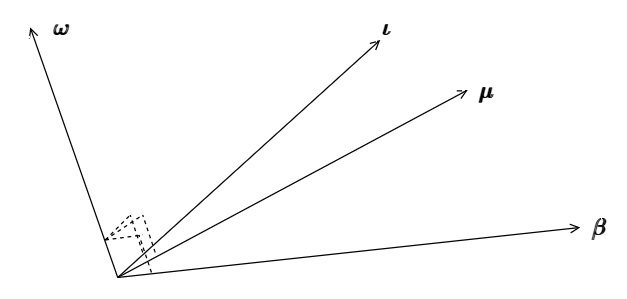
\includegraphics[width=0.6\textwidth]{fig/apt.jpg}
    \caption{APT}
    \label{fig:apt}
\end{figure}

因此在数学上,资产预期收益率$\bm{\mu}$可以写成$\bm{1}$与$\bm{\beta}$的线性组合,即:
\begin{equation*}
    \bm{\mu} = \gamma_1 \bm{1} + \gamma_2 \bm{\beta}
\end{equation*}

那么此时上式应对任何资产都成立,为了求解$\gamma_1$与$\gamma_2$可代入特殊资产,无风险资产($R_f$),与市场组合($R_M$)。由于无风险资产的因子暴露为零,代入上式可得:
\begin{equation*}
    R_f = \gamma_1
\end{equation*}

对于市场组合,其$beta=1$,并将$\gamma_1 = R_f$代入,可得:
\begin{equation*}
    R_M = R_f + \gamma_2 \times \bm{1}
\end{equation*}

因此有:
\begin{equation*}
    \gamma = R_M - R_f
\end{equation*}

代入原式,最终可得到CAPM的表达式:
\begin{equation*}
    \mu_i = R_f + \beta_i(R_M - R_f)
\end{equation*}

在此基础上,扩展至多因子,即得到APT模型:
\begin{equation*}
    \E[R_{i}^{e}] = \mu_i - R_f = \beta_{i,1} \lambda_1 + \beta_{i,2} \lambda_2 + \dots + \beta_{i,K} \lambda_K
\end{equation*}

\end{appendices}

\end{document}